For this case, the numerical simulation is performed for a real 
coronary artery with atherosclerosis whose geometry was obtained 
through an image processing as suggested by Wang et al. (2017) 
\cite{wang2017}. This geometry is particular to each patient 
due to the patient health conditions. As in the previous case, 
the stent strut was modeled by
10 uniformly spaced semi-circles.
The domain was discretized using 11807 nodes and 26426 linear 
triangular elements. 

\medskip
The \ref{velocity evolution real stent} shows the unsteady state velocity 
profile in the section where the horizontal velocity 
has the maximum non-dimensional value.
In this case, the section is different than the previous one
and its value is $x=6.65R$. 
Even so, the numerical solution shown a simular
profile to the previous case and
as we can see, the maximum non-dimensional value of the velocity field 
reaches $u=3.68$ close to symmetric axis. 
However, this velocity may vary according to the 
coronary artery geometry for each patient.
It compared to the curved channel, the maximum horizontal velocity
had an increase of $5.14\%$. Therefore, the curved channel
shown an acceptable approach,
besides this model being simpler to implement
and to perform the numerical simulations than real channel model.


\begin{figure}[H]
     \centering
     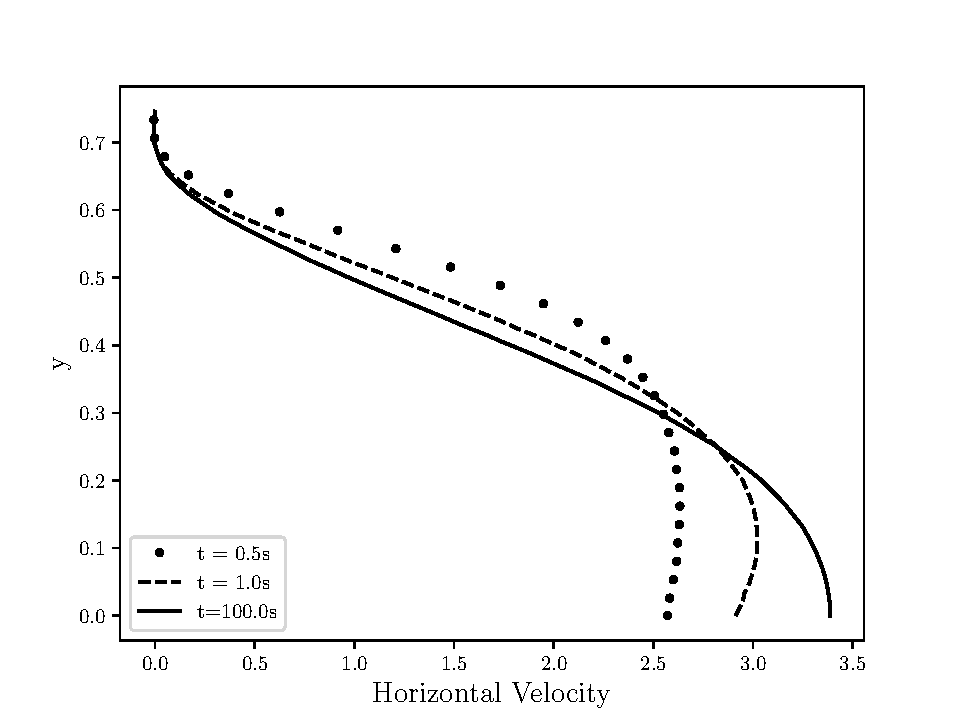
\includegraphics[scale=1]{./02_chaps/cap_solution/figure/vel_RealStrut_evol.pdf}\\
     \caption{
The steady state velocity profile for real channel with drug-eluting stent.}
     \label{velocity evolution real stent}
\end{figure}

\medskip
The \ref{velocity field real stent} presents the evolution in 
time and space of the velocity field for half of the domain. 
The velocity field is represented with non-dimensional values 
where the red color refers to the $u=3.68$ value and the blue color 
$u=0$ value. Conveting to dimensional values, 
we have $u=44.2cm/s$ and $u=0cm/s$ respectively. As in the previous case,
the region with the lowest horizontal velocity magnitue is found close to
the boundary due to the no-slip
condition and the largest horizontal
velocity value is found close to
symmetric axis. For this real channel, is possible to observe that
there is two contraction region where
the velocity field is increased.
However, this coronary artery geometry varies for each patient and its blood dynamics can be changed.


\vspace{2cm} 
\begin{figure}[H]
     \begin{minipage}{.50\linewidth}
      \centering
      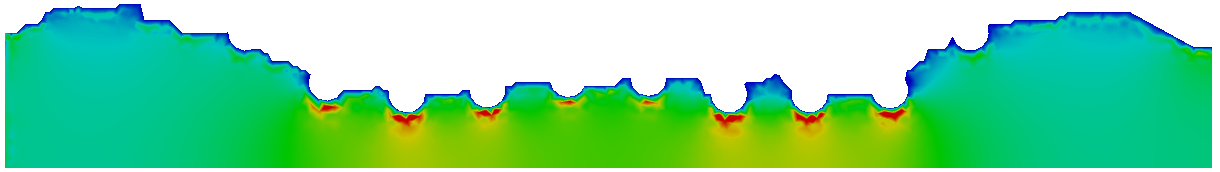
\includegraphics[scale=0.18]{./02_chaps/cap_solution/figure/vel_RealStrut1.png}\\
      t = 0.1s
     \end{minipage}%
     \begin{minipage}{.50\linewidth}
      \centering
      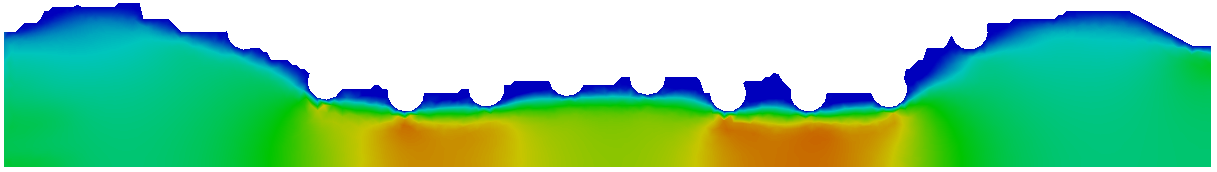
\includegraphics[scale=0.18]{./02_chaps/cap_solution/figure/vel_RealStrut2.png}\\
      t = 0.5s
     \end{minipage}
     \begin{minipage}{.50\linewidth}
     \medskip
      \centering
      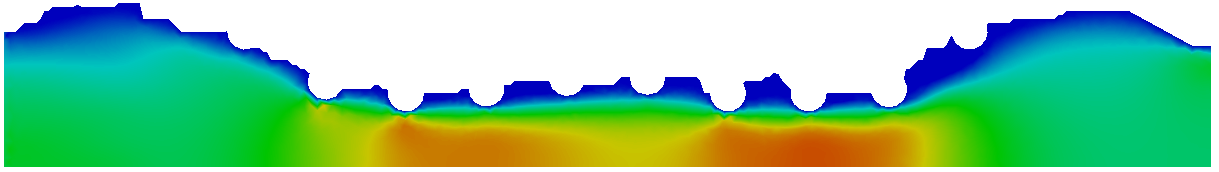
\includegraphics[scale=0.18]{./02_chaps/cap_solution/figure/vel_RealStrut3.png}\\
      t = 1.0s
     \end{minipage}%
     \begin{minipage}{.50\linewidth}
     \medskip
      \centering
      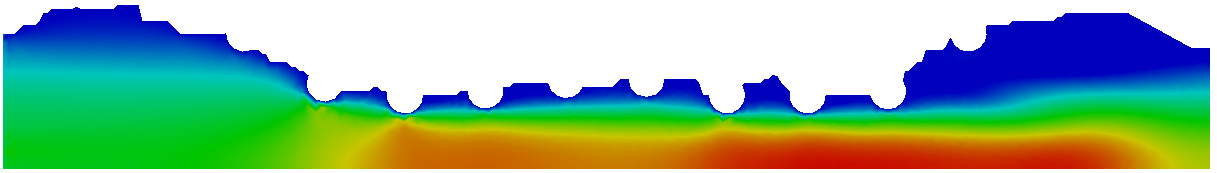
\includegraphics[scale=0.18]{./02_chaps/cap_solution/figure/vel_RealStrut4.png}\\
      t = 3.0s
     \end{minipage}
     \begin{minipage}{.50\linewidth}
      \centering
      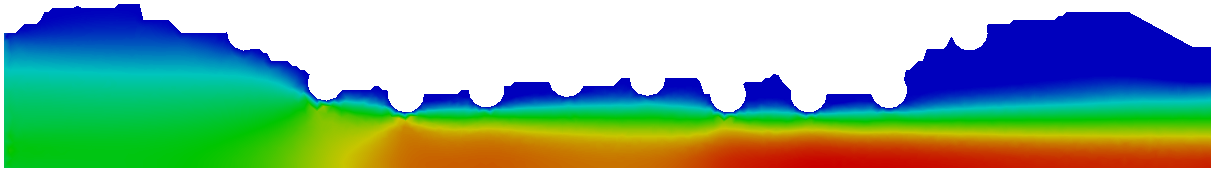
\includegraphics[scale=0.18]{./02_chaps/cap_solution/figure/vel_RealStrut5.png}\\
      t = 5.0s
     \end{minipage}%
     \begin{minipage}{.50\linewidth}
      \centering
      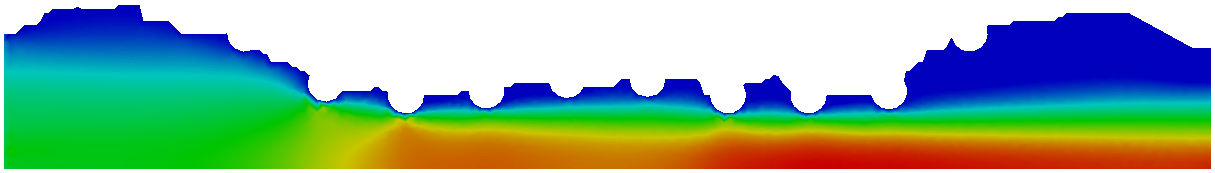
\includegraphics[scale=0.18]{./02_chaps/cap_solution/figure/vel_RealStrut6.png}\\
      t = 7.0s
     \end{minipage}
     \begin{minipage}{.50\linewidth}
     \medskip
      \centering
      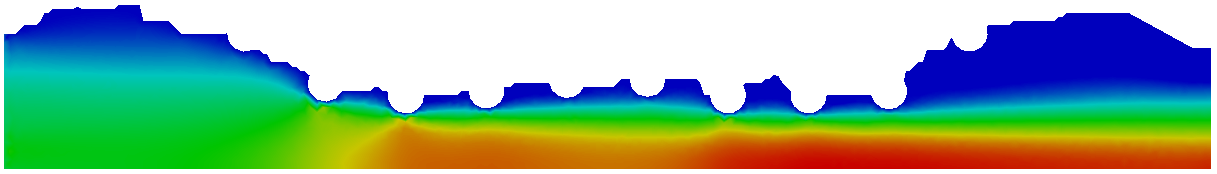
\includegraphics[scale=0.18]{./02_chaps/cap_solution/figure/vel_RealStrut7.png}\\
      t = 10.0s
     \end{minipage}%
     \begin{minipage}{.50\linewidth}
     \medskip
      \centering
      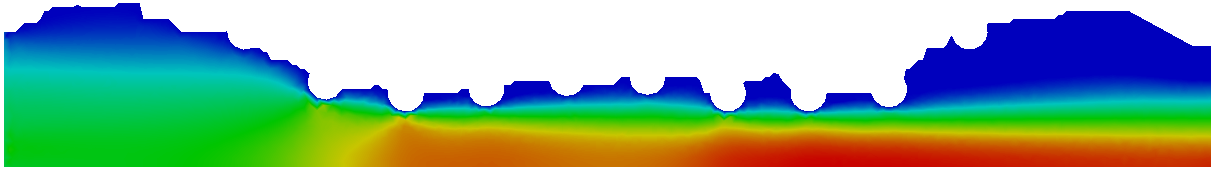
\includegraphics[scale=0.18]{./02_chaps/cap_solution/figure/vel_RealStrut8.png}\\
      t = 100.0s
     \end{minipage}\\[10pt]
      \centering
      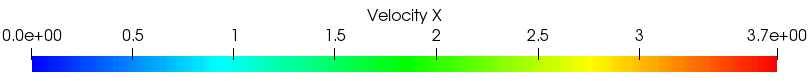
\includegraphics[scale=0.5]{./02_chaps/cap_solution/figure/vel_RealStrutScale.png}\\
     \medskip
     \caption{
Temporal and spatial evolution of the velocity field for real channel with
drug-eluting stent.}
     \label{velocity field real stent}
\end{figure}





\vspace{1cm}
The \ref{conc field real stent sc 1} to
\ref{conc field real stent sc 1000} show the temporal and spatial evolution 
of the concentration field for several \textit{Schmidt} number, 
such as: $1$, $10$, $100$ and $1000$ respectively. The concentration field is 
represented with the non-dimensional values where the red color 
represents $100$\% and the blue color represents $0$\% 
of the diffused concentration in the bloodstream. 
It is possible to observe that the concentration field dynamic
is similar than the curved channel, no significant differences
from the previous one for each Schmidt number.
Only in some regions that the concentration field
become more diffuse as a consequence of the velocity 
field decrease due to irregular geometry close to the
semi-circles of the stents.


\begin{figure}[H]
     \begin{minipage}{.50\linewidth}
      \centering
      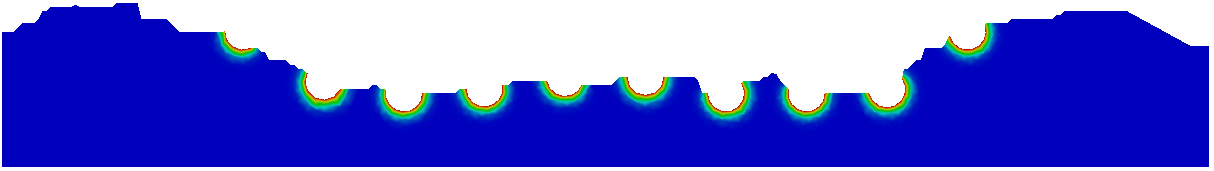
\includegraphics[scale=0.18]{./02_chaps/cap_solution/figure/conc1_RealStrut1.png}\\
      t = 0.1s
     \end{minipage}%
     \begin{minipage}{.50\linewidth}
      \centering
      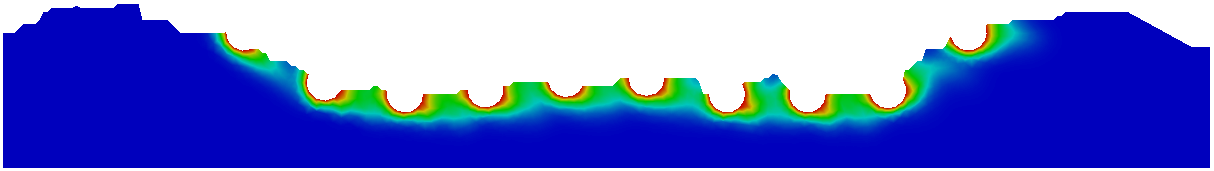
\includegraphics[scale=0.18]{./02_chaps/cap_solution/figure/conc1_RealStrut2.png}\\
      t = 0.5s
     \end{minipage}
     \begin{minipage}{.50\linewidth}
     \medskip
      \centering
      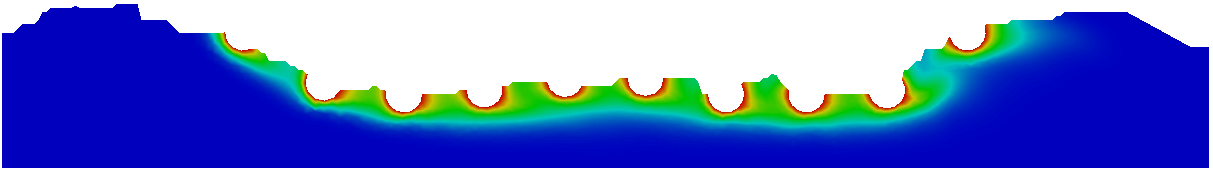
\includegraphics[scale=0.18]{./02_chaps/cap_solution/figure/conc1_RealStrut3.png}\\
      t = 1.0s
     \end{minipage}%
     \begin{minipage}{.50\linewidth}
     \medskip
      \centering
      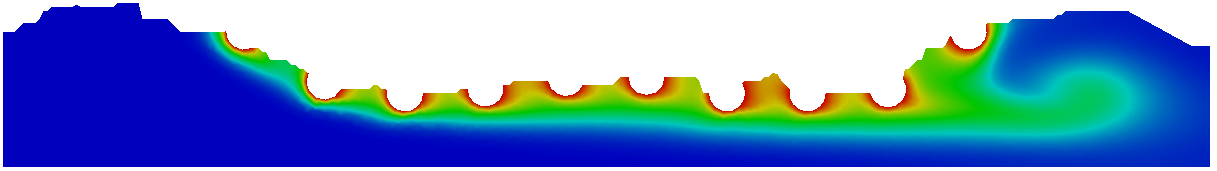
\includegraphics[scale=0.18]{./02_chaps/cap_solution/figure/conc1_RealStrut4.png}\\
      t = 3.0s
     \end{minipage}
     \begin{minipage}{.50\linewidth}
      \centering
      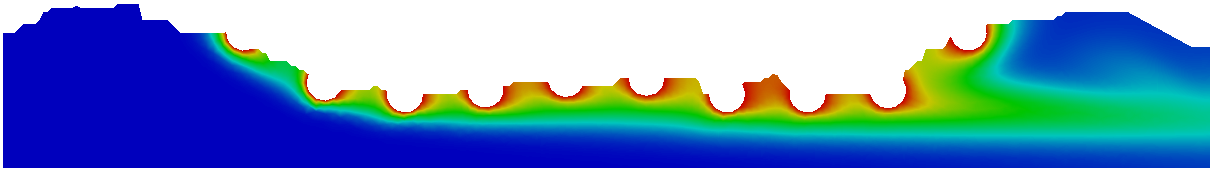
\includegraphics[scale=0.18]{./02_chaps/cap_solution/figure/conc1_RealStrut5.png}\\
      t = 5.0s
     \end{minipage}%
     \begin{minipage}{.50\linewidth}
      \centering
      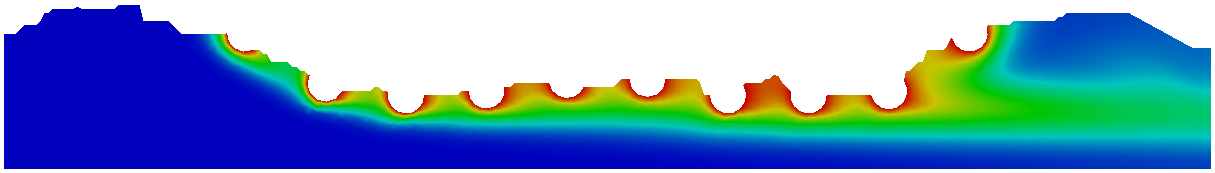
\includegraphics[scale=0.18]{./02_chaps/cap_solution/figure/conc1_RealStrut6.png}\\
      t = 7.0s
     \end{minipage}
     \begin{minipage}{.50\linewidth}
     \medskip
      \centering
      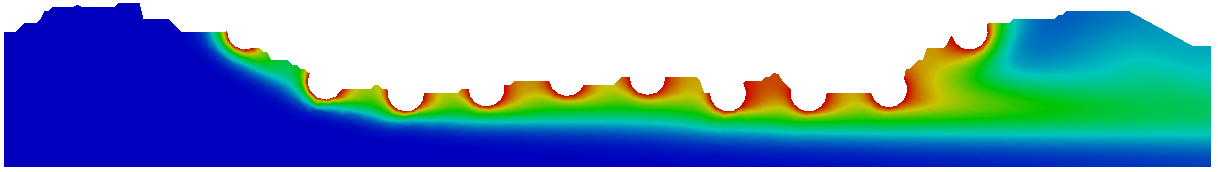
\includegraphics[scale=0.18]{./02_chaps/cap_solution/figure/conc1_RealStrut7.png}\\
      t = 10.0s
     \end{minipage}%
     \begin{minipage}{.50\linewidth}
     \medskip
      \centering
      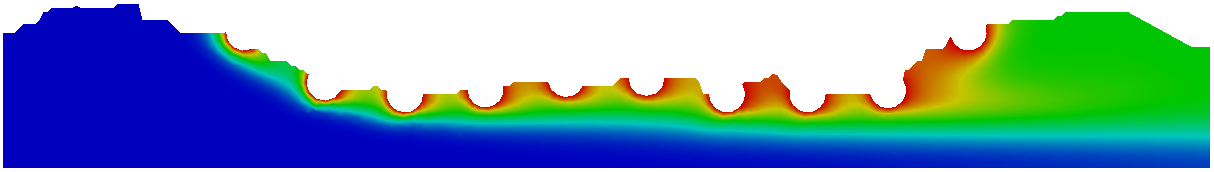
\includegraphics[scale=0.18]{./02_chaps/cap_solution/figure/conc1_RealStrut8.png}\\
      t = 100.0s
     \end{minipage}\\[10pt]
      \centering
      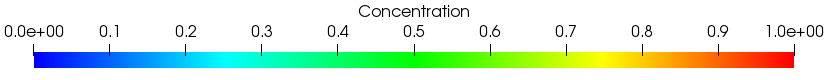
\includegraphics[scale=0.5]{./02_chaps/cap_solution/figure/conc1_RealStrutScale.png}\\
     \medskip
     \caption{
Temporal and spatial evolution of the concentration fiel for real channel with drug-eluting stent and $Sc=1$.}
     \label{conc field real stent sc 1}
\end{figure}



\begin{figure}[H]
     \begin{minipage}{.50\linewidth}
      \centering
      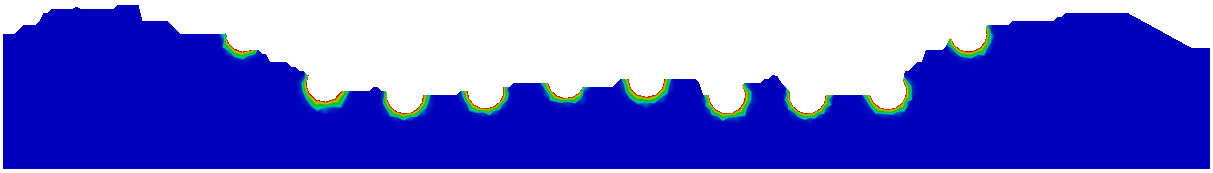
\includegraphics[scale=0.18]{./02_chaps/cap_solution/figure/conc10_RealStrut1.png}\\
      t = 0.1s
     \end{minipage}%
     \begin{minipage}{.50\linewidth}
      \centering
      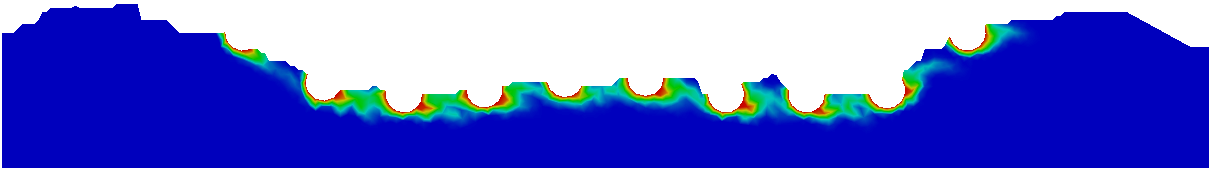
\includegraphics[scale=0.18]{./02_chaps/cap_solution/figure/conc10_RealStrut2.png}\\
      t = 0.5s
     \end{minipage}
     \begin{minipage}{.50\linewidth}
     \medskip
      \centering
      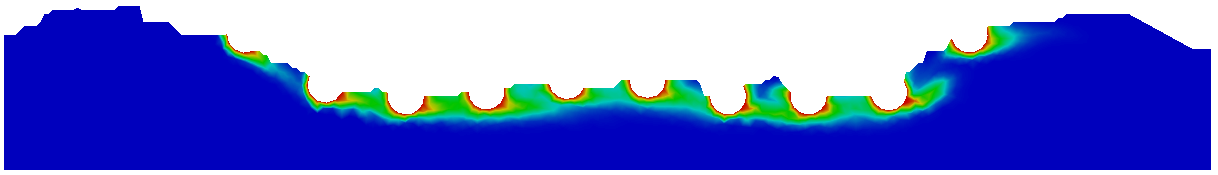
\includegraphics[scale=0.18]{./02_chaps/cap_solution/figure/conc10_RealStrut3.png}\\
      t = 1.0s
     \end{minipage}%
     \begin{minipage}{.50\linewidth}
     \medskip
      \centering
      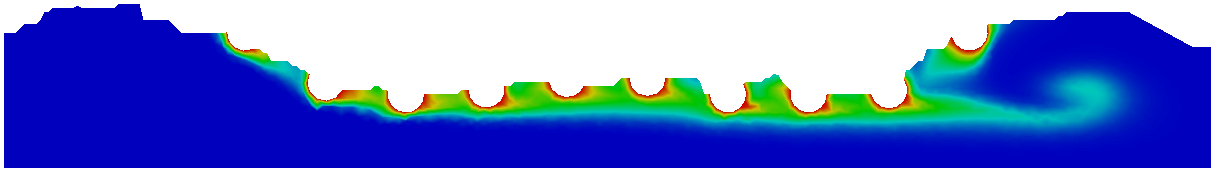
\includegraphics[scale=0.18]{./02_chaps/cap_solution/figure/conc10_RealStrut4.png}\\
      t = 3.0s
     \end{minipage}
     \begin{minipage}{.50\linewidth}
      \centering
      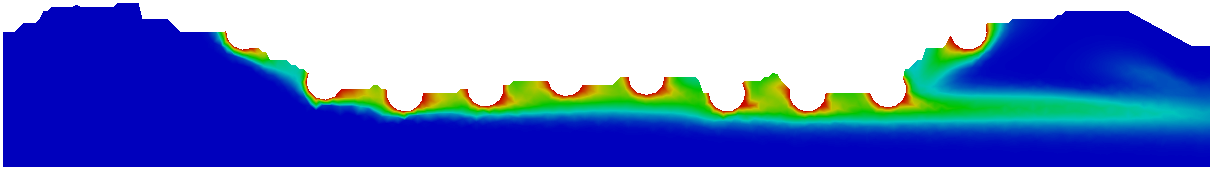
\includegraphics[scale=0.18]{./02_chaps/cap_solution/figure/conc10_RealStrut5.png}\\
      t = 5.0s
     \end{minipage}%
     \begin{minipage}{.50\linewidth}
      \centering
      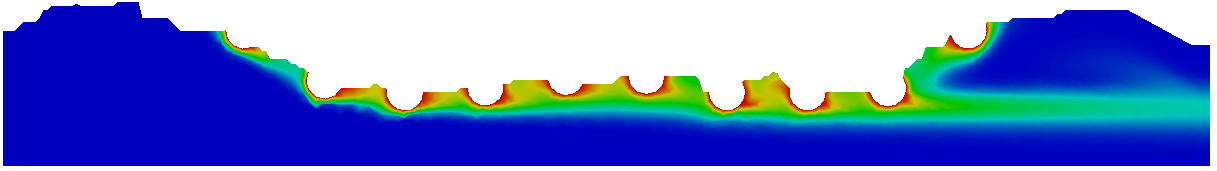
\includegraphics[scale=0.18]{./02_chaps/cap_solution/figure/conc10_RealStrut6.png}\\
      t = 7.0s
     \end{minipage}
     \begin{minipage}{.50\linewidth}
     \medskip
      \centering
      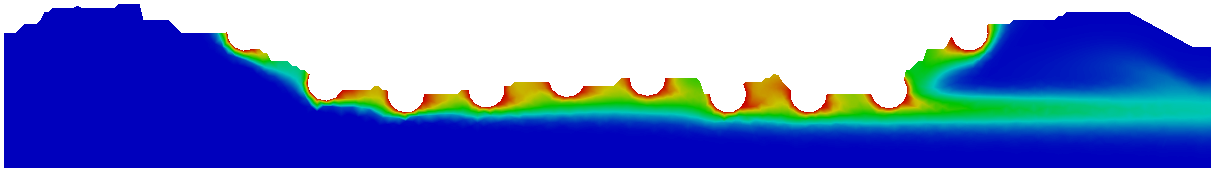
\includegraphics[scale=0.18]{./02_chaps/cap_solution/figure/conc10_RealStrut7.png}\\
      t = 10.0s
     \end{minipage}%
     \begin{minipage}{.50\linewidth}
     \medskip
      \centering
      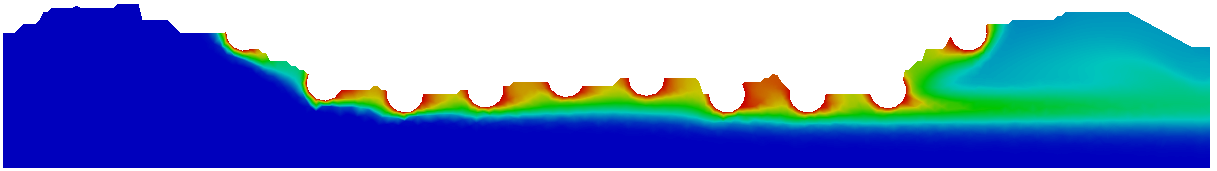
\includegraphics[scale=0.18]{./02_chaps/cap_solution/figure/conc10_RealStrut8.png}\\
      t = 100.0s
     \end{minipage}\\[10pt]
      \centering
      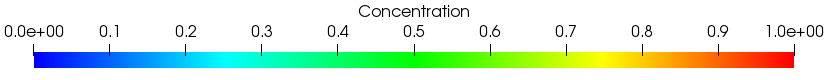
\includegraphics[scale=0.5]{./02_chaps/cap_solution/figure/conc1_RealStrutScale.png}\\
     \medskip
    \caption{
Temporal and spatial evolution of the concentration fiel for real channel with drug-eluting stent and $Sc=10$.}
     \label{conc field real stent sc 10}
\end{figure}



\begin{figure}[H]
     \begin{minipage}{.50\linewidth}
      \centering
      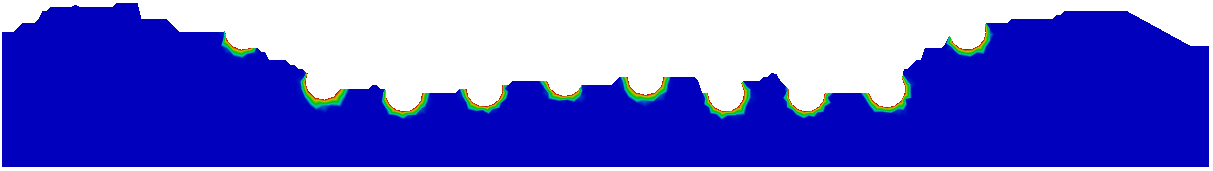
\includegraphics[scale=0.18]{./02_chaps/cap_solution/figure/conc100_RealStrut1.png}\\
      t = 0.1s
     \end{minipage}%
     \begin{minipage}{.50\linewidth}
      \centering
      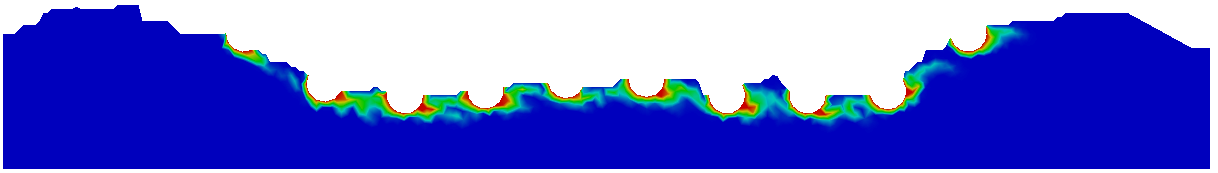
\includegraphics[scale=0.18]{./02_chaps/cap_solution/figure/conc100_RealStrut2.png}\\
      t = 0.5s
     \end{minipage}
     \begin{minipage}{.50\linewidth}
     \medskip
      \centering
      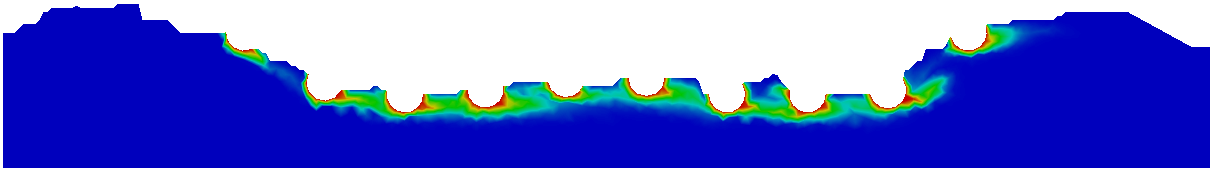
\includegraphics[scale=0.18]{./02_chaps/cap_solution/figure/conc100_RealStrut3.png}\\
      t = 1.0s
     \end{minipage}%
     \begin{minipage}{.50\linewidth}
     \medskip
      \centering
      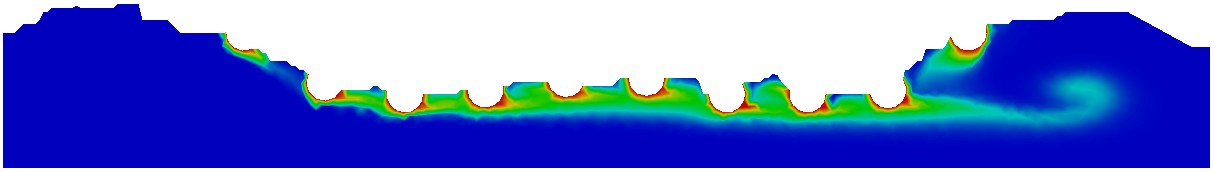
\includegraphics[scale=0.18]{./02_chaps/cap_solution/figure/conc100_RealStrut4.png}\\
      t = 3.0s
     \end{minipage}
     \begin{minipage}{.50\linewidth}
      \centering
      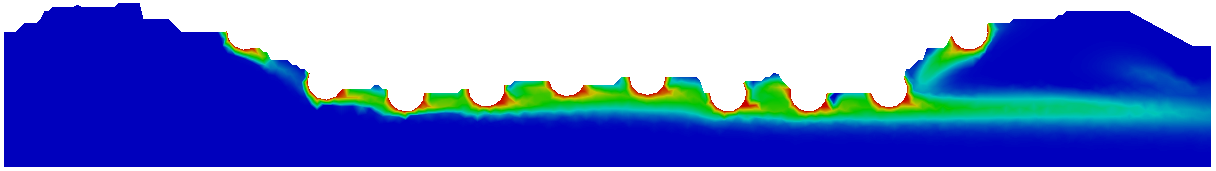
\includegraphics[scale=0.18]{./02_chaps/cap_solution/figure/conc100_RealStrut5.png}\\
      t = 5.0s
     \end{minipage}%
     \begin{minipage}{.50\linewidth}
      \centering
      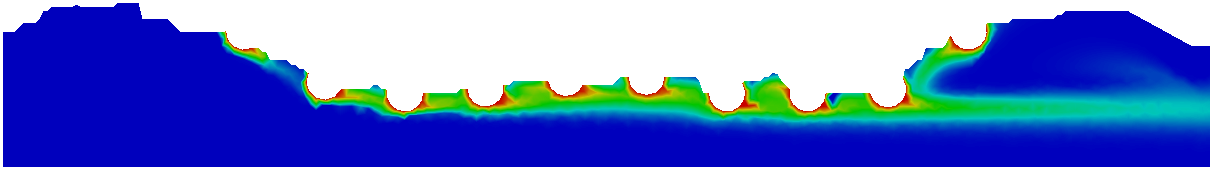
\includegraphics[scale=0.18]{./02_chaps/cap_solution/figure/conc100_RealStrut6.png}\\
      t = 7.0s
     \end{minipage}
     \begin{minipage}{.50\linewidth}
     \medskip
      \centering
      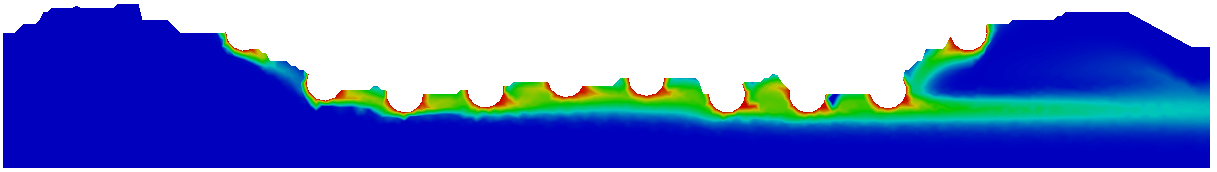
\includegraphics[scale=0.18]{./02_chaps/cap_solution/figure/conc100_RealStrut7.png}\\
      t = 10.0s
     \end{minipage}%
     \begin{minipage}{.50\linewidth}
     \medskip
      \centering
      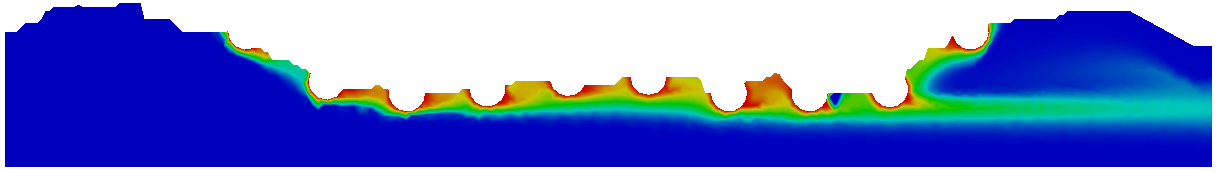
\includegraphics[scale=0.18]{./02_chaps/cap_solution/figure/conc100_RealStrut8.png}\\
      t = 100.0s
     \end{minipage}\\[10pt]
      \centering
      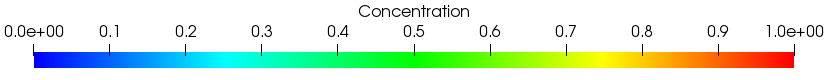
\includegraphics[scale=0.5]{./02_chaps/cap_solution/figure/conc1_RealStrutScale.png}\\
     \medskip
    \caption{
Temporal and spatial evolution of the concentration fiel for real channel with drug-eluting stent and $Sc=100$.}
     \label{conc field real stent sc 100}
\end{figure}


\begin{figure}[H]
     \begin{minipage}{.50\linewidth}
      \centering
      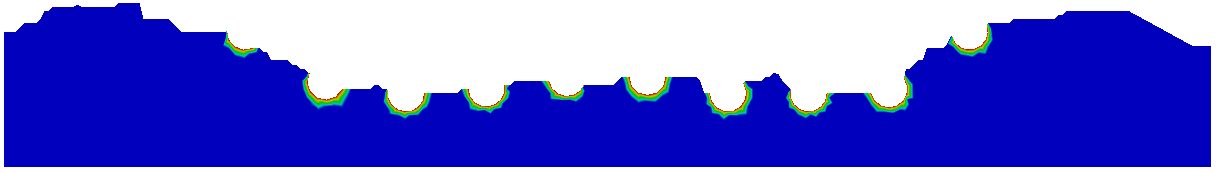
\includegraphics[scale=0.18]{./02_chaps/cap_solution/figure/conc1000_RealStrut1.png}\\
      t = 0.1s
     \end{minipage}%
     \begin{minipage}{.50\linewidth}
      \centering
      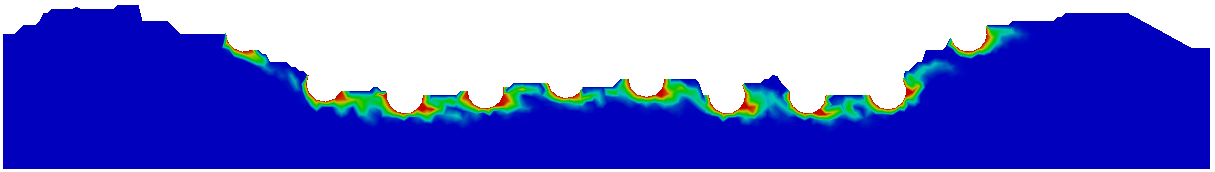
\includegraphics[scale=0.18]{./02_chaps/cap_solution/figure/conc1000_RealStrut2.png}\\
      t = 0.5s
     \end{minipage}
     \begin{minipage}{.50\linewidth}
     \medskip
      \centering
      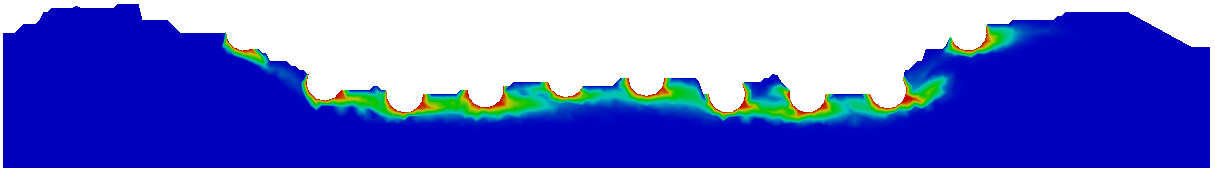
\includegraphics[scale=0.18]{./02_chaps/cap_solution/figure/conc1000_RealStrut3.png}\\
      t = 1.0s
     \end{minipage}%
     \begin{minipage}{.50\linewidth}
     \medskip
      \centering
      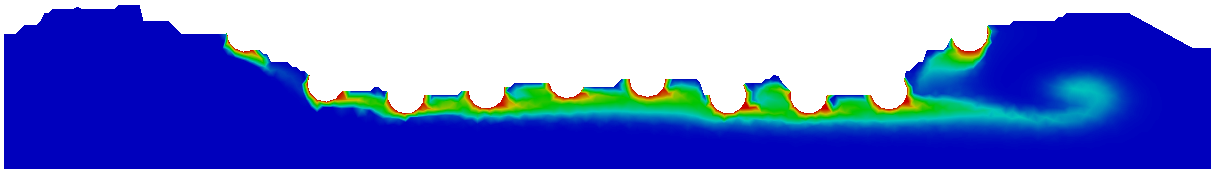
\includegraphics[scale=0.18]{./02_chaps/cap_solution/figure/conc1000_RealStrut4.png}\\
      t = 3.0s
     \end{minipage}
     \begin{minipage}{.50\linewidth}
      \centering
      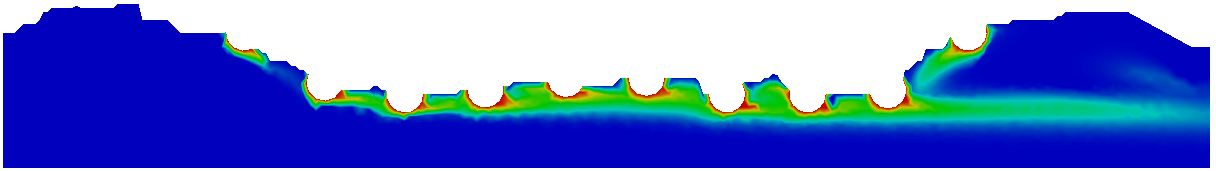
\includegraphics[scale=0.18]{./02_chaps/cap_solution/figure/conc1000_RealStrut5.png}\\
      t = 5.0s
     \end{minipage}%
     \begin{minipage}{.50\linewidth}
      \centering
      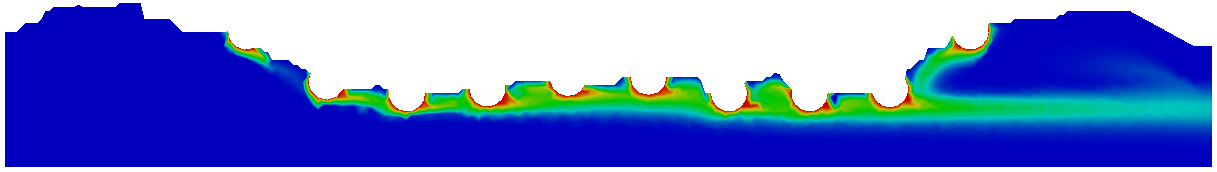
\includegraphics[scale=0.18]{./02_chaps/cap_solution/figure/conc1000_RealStrut6.png}\\
      t = 7.0s
     \end{minipage}
     \begin{minipage}{.50\linewidth}
     \medskip
      \centering
      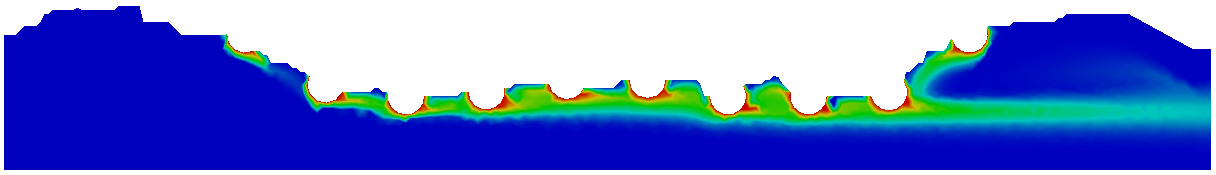
\includegraphics[scale=0.18]{./02_chaps/cap_solution/figure/conc1000_RealStrut7.png}\\
      t = 10.0s
     \end{minipage}%
     \begin{minipage}{.50\linewidth}
     \medskip
      \centering
      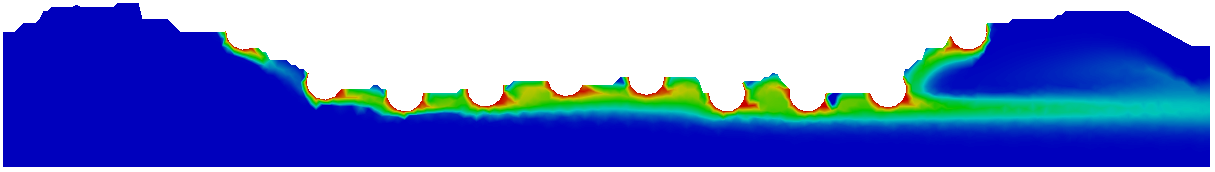
\includegraphics[scale=0.18]{./02_chaps/cap_solution/figure/conc1000_RealStrut8.png}\\
      t = 100.0s
     \end{minipage}\\[10pt]
      \centering
      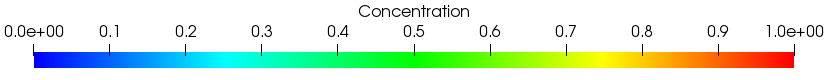
\includegraphics[scale=0.5]{./02_chaps/cap_solution/figure/conc1_RealStrutScale.png}\\
     \medskip
    \caption{
Temporal and spatial evolution of the concentration fiel for real channel with drug-eluting stent and $Sc=1000$.}
     \label{conc field real stent sc 1000}
\end{figure}




\newpage


